\documentclass{article}
\usepackage{tikz}
\begin{document}
We are working on 
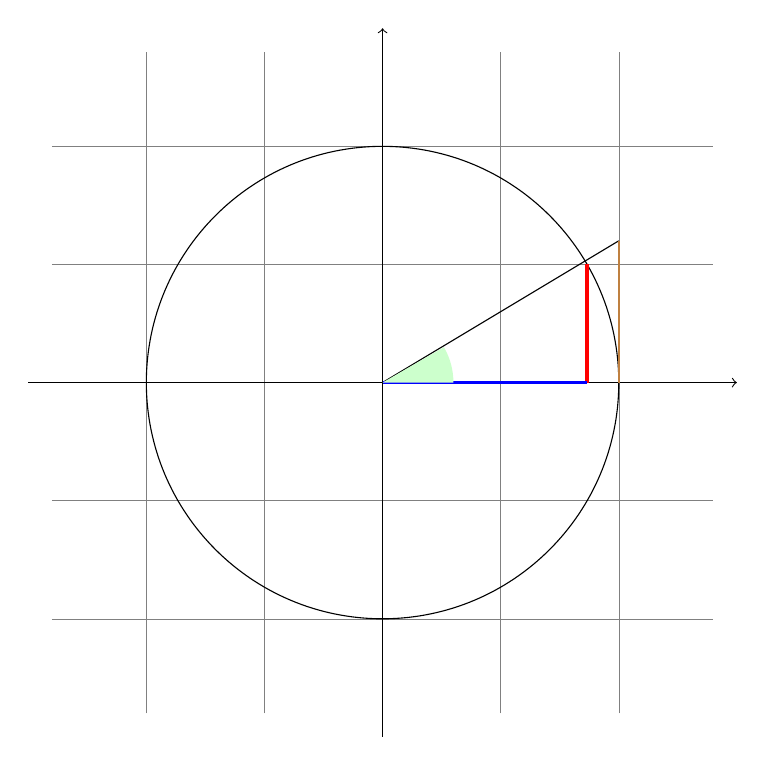
\begin{tikzpicture}[scale = 3]
% We use \clip command to focus a specific part of a picture.
    % \clip (-0.1,-0.2) rectangle (1.1,0.75);

    % \draw [step = 0.5cm, help lines] (-1.4, -1.4) grid (1.4, 1.4);
    \draw [step = 0.5cm, very thin, gray] (-1.4, -1.4) grid (1.4, 1.4);
    \draw [->] (-1.5, 0) -- (1.5, 0);
    \draw [->] (0, -1.5) -- (0, 1.5);

% We can make the Center Circle using Bezier Curves/ Curved Path Construction.
%     \draw (-1, 0) .. controls (-1, 0.555) and (-0.555, 1) .. (0, 1);
%     \draw (0, 1) .. controls (0.555, 1) and (1, 0.555) .. (1, 0);
% But it is easier is use Circle Path Construction.

    \draw (0, 0) circle [radius = 1cm];

% We can make the grid usig Recangle Path Construction.
    % \draw (0, 0) rectangle (0.5, 0.5);
    % \draw (0, 0) rectangle (-0.5, -0.5);
% But the easier process is direct use Grid Path Construction.

    \draw (0, 0) -- (1, 0.6);
    \draw [brown, line width = 0.6] (1, 0) -- (1, 0.6);
    \draw [red, very thick] (30 : 1cm) -- +(0, -0.5);
    \draw [blue, very thick] (30 : 1cm) ++ (0, -0.5) -- (0, 0);

% The angle sign have to be draw by arc.

    % \draw (3mm, 0mm) arc [start angle = 0, end angle = 30, radius = 3mm];
    \fill [green!20!white] (0, 0) -- (3mm, 0mm)
        arc [start angle = 0, end angle = 30, radius = 3mm] -- (0, 0);
    
\end{tikzpicture}

% Extra Work

% \tikz{
%     \draw (-1.5, 0) -- (1.5, 0);
%     \draw (1.5, 0) -- (0, -1.5);
%     \draw (0, -1.5) -- (0, 1.5);
% }

% \begin{tikzpicture}
% Curve
%     \filldraw [gray] (0,0) circle [radius=2pt]
%     (1,1) circle [radius=2pt]
%     (2,1) circle [radius=2pt]
%     (2,0) circle [radius=2pt];
%     \draw (0,0) .. controls (1,1) and (2,1) .. (2,0);
% Ellipse
%     \draw (0,0) ellipse [x radius=20pt, y radius=10pt];
% \end{tikzpicture}

\end{document}
\bye